\documentclass[twocolumn,amsmath,superscriptaddress,amssymb]{revtex4-1}

\usepackage{ulem}
\usepackage[usenames]{color}
\usepackage{epsfig}
\usepackage{graphicx}
\usepackage{times}
\usepackage{dcolumn}
%\usepackage{slashbox,pict2e}
\usepackage[colorlinks=false, hidelinks ]{hyperref}
\usepackage{grfext}

\bibliographystyle{siam}
\renewcommand{\thefootnote}{\fnsymbol{footnote}}
\renewcommand{\figurename}{}
\renewcommand{\thefigure}{Fig.\arabic{figure}}
\renewcommand{\theequation}{Eq.\arabic{equation}}
\renewcommand{\thesection}{\arabic{section}}
%\pagestyle{empty}


\newcommand{\vect}[1]{\boldsymbol{#1}}
\newcommand{\angstrom}{\textup{\AA}}
\graphicspath{ {./Graphics/} }
\DeclareGraphicsExtensions{.png,.pdf,.jpg}

\let\vec\mathbf

\begin{document}
\title{Resonant Inelastic X-ray Spectroscopy on $LiCu_3 O_3$ }
\author{ R. \'{S}wi\c{e}tek}\affiliation{Wrocław University of Science and Technology, Wroc\l{}aw 50-370, Poland}
\author{ S. Moser}\affiliation{Physikalisches Institut, Universit\"{a}t W\"{u}rzburg, D-97074 W\"{u}rzburg, Germany}\affiliation{Advanced Light Source, E. O. Lawrence Berkeley National Laboratory, Berkeley, California 94720,USA}
%\date{\today} % Leave empty to omit a date
\begin{abstract}
In this paper we investigate the resonant inelastic Soft X-ray spectra (RIXS) of $LiCu_3O3$ on the copper $ L_{2,3}$ edges for determination of optical properties of the material including intermediate dd exciation in the RIXS experiment. Various copper compunds exhibits a strong magnetic responce, whether ferromagnetic or antiferromagnetic, which is also the case in this material. It consists of 4 layers in the unit cell: 2 layers with $CuO$ and 2 layers $Cu^{1+}$ with randomly substituted lithium for copper (II) atoms. We have a look onto the optical spectra mentioned before and the x-ray absorption spectra. We further analyze the magnetic behaviour in terms of circular and linear magnetic dichroism. 
\end{abstract}
\maketitle
%----------------------------------------INTRODUCTION-------------------------------------------------------
\section{Introduction}

In the past recent years there is a continuous growth in interest of developing new techniques of probing magnetic properties of transition metal (TM) compundsand rare earths (RE). Usually one would use the standard inelastic neutron scattering (INS) technique, but in the following paper we will show you an equivalent way using resonant inelastic x-ray scattering (RIXS) measurments. They show a significant feature, namely one can directly extract the whole complex refractive index $n_c = 1-\delta + i\kappa$ with no need of using the Kramers-Kronig transformations \cite{Llosa,Emeis}. Moreover the consistency of this relations (and its extensions for small energy ranges) is being investigated in this paper. \\
\indent Depending on the oxidation state of copper we have an unfilled 3d shell (for $Cu^{2+}$) or a completely filled one (for $Cu^{1+}$). This means the $CuO$ planes in the crystals exhibit the magnetic ordering, while the $Cu^{1+}$ doesn't affect the magnetic structure at all. The structure of the unit cell is shown in \ref{UnitCell}. The lattice has a tetragonal $P4/mmm$ structure with lattice parameters $a=2.81\angstrom$ and $c=8.90\angstrom$, which result in corresponding symmetries in the optical conductivity tensor. Crystal symmetries and their effect on the scattering amplitude of a crystal are thoroughly considered in \cite{Haverkort2}. Using those analysis for the symmetry of our crystal we can directly extract the complex conductivity tensor (see appendix C). These result gives us sufficient data for characterizing ther material in terms of optical properties.\\
\indent Most cupprates exhibits antiferromagnetic ordering (some resulting in superconducting states, like $LaCu_2O_4$), which can result in spin flip excitations and thus magnon creation \cite{Haverkort}. The magnon dispersion can be extracted from the RIXS data, if only one could filter those excitations. In this experiment all possible excitations in the given energy range are detected, thus to have the desired magnon dispersion one needs to substract all other influences. This can be done having the conductivity tensor, namely the RIXS intensity can be viewed as:
\begin{equation}
I_{RIXS}\varpropto\left|\vec{e}_{out}^*\omega\tensor{\sigma}\vec{e}_{in}\right|, 
\end{equation}
\noindent where $\vect{e}_{in}$($\vect{e}_{out}$)  is the incidence(scattered) wave polarization.
%----CRYSTAL -----
\begin{figure}[t!]
        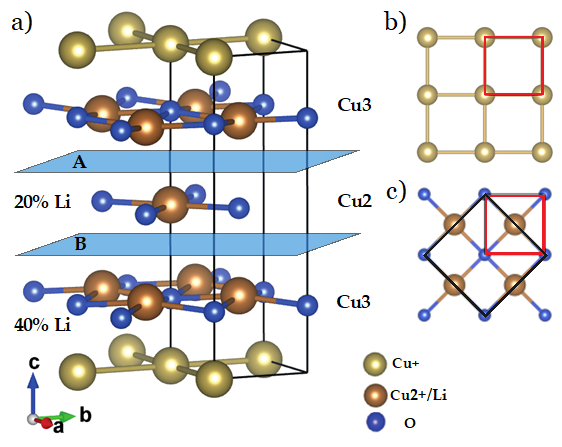
\includegraphics[width=0.85\columnwidth, height = 6 cm]{UnitCell.png}
\caption{(a) Structure of the unit cell of $LiCu_3O_3$, 3 planes of $CuO$ are sandwiched between $Cu^{+1}$ planes. Pictures (b) and (c) show the $CuO$ and $Cu^{1+}$ planes respectively. }
\label{UnitCell} 
\end{figure}
It remains to properly guess (or model) the scattered polarization using symmetry arguments. One can average the RIXS intensity for every possible superposition of the scattered polarization, but one the other hand a competent weighting factor would be needed.  Another possibility is to assume no change of the polarization state (only rotation of the polarization vector) to determine from the conductivity tensor the RIXS spectrum assosiated with dipole transitions. However one can argue that the re excitation proces is independent on the exciton generation and thus shouldn't be dependent on the incident polarization. This means every polarization (allowed by the symmetry) should be allowed, regardless to the incoming wave polarization.
%
%----------------------------------------THEORY-------------------------------------------------------
\section{Theoretical background}
The core understanding in x-ray spectroscopies lies in the us of sceond-order perturbation theory with a interaction hamiltonian directly related to the vector potential of the incoming wave. In general neglecting the interactionn bewtween electrons one can show that the vector potential $\vect{A}(\vect{r})$ enters the hamiltonian through the kinematic part of the energy, namely:
\begin{equation}\label{eq: hamil}
\hat{H} = \sum_i\frac{(\vect{p}_i-e\vect{A}_i)^2}{2m_i},
\end{equation}
%
\noindent where $\vect{p}_i$ and $m_i$ are the momentum and mass of the i-th electron. Considering the interaction of the electrons, the ligand field and making use of Fermi's goldern rule one can obtain the RIXS amplitude as \cite{PasqualephD}:
%
\begin{equation}\label{eq: Kramer Heisenberg}
\begin{split}
\frac{d^2\sigma}{d\omega d\Omega}=\sum_f\left|\sum_n\frac{\langle f|\hat{\vect{D}}_{out}^{\dag}|n\rangle \langle n|\hat{\vect{D}}_{in}|i\rangle}{E_g+\hslash\omega-E_n+i\Gamma}\right|^2\\
\times\delta(\hslash\omega-\hslash\omega'+E_g-E_f),
\end{split}
\end{equation}
%
\noindent where $\omega$ and $\omega'$ are the frequencies of the incoming and outgoing wave, $\hat{\vect{D}}_\nu = \vect{e}_\nu\cdot\hat{\vect{p}}~exp(\pm \vect{k}_\nu \cdot \vect{r})$ is the dipole transition operator ($\nu=in,out$) with $\vect{k}_{in}$($\vect{k}_{out}$) being the wave vector of the incident(scattered) wave (see appendix A and B). The ground, intermediate and final states are denoted as $|i\rangle$, $|n\rangle$ and $|f\rangle$ respectively, where the sum is taken out over all intermediate and final states. The corresponding energies to these states are: $E_i$, $E_n$ and $E_f$. The \ref{Process} shows the common RIXS process, which involves core hole-electron coulomb interaction, causing the creation of a hole in the valence shell. The initial state and the final state doesn't need to be necessarily be the same, various intermediate interactions can change the final state\\
\indent To consider properly the excitation of core electrons one needs to look at the allowed transitions using selection rules governed by the crystal symmetry. For the case of $Cu^{2+}$ we have a hole in the $d_{x^2-y^2}$ orbital. It is clear that in such an unoccupied state one cannot excite a $p_z$ electrons (in the dipole approximation) due to the selection rules. The dipole allowed transtiotions are deiscribed by the change in the orbital momentum by $\Delta\ell= 0,\pm1$ (this proves the previous statement). In contrast the quadrupole transition allows excitation with $\Delta\ell= \pm2$, thus the excitation of $p_z$ electron into the $d_{x^2-y^2}$ are allowed. However in most cupprates and other early TM such transitions are of low magnitude compared to the dipole transition.\\
%
\begin{figure}[tp!]
        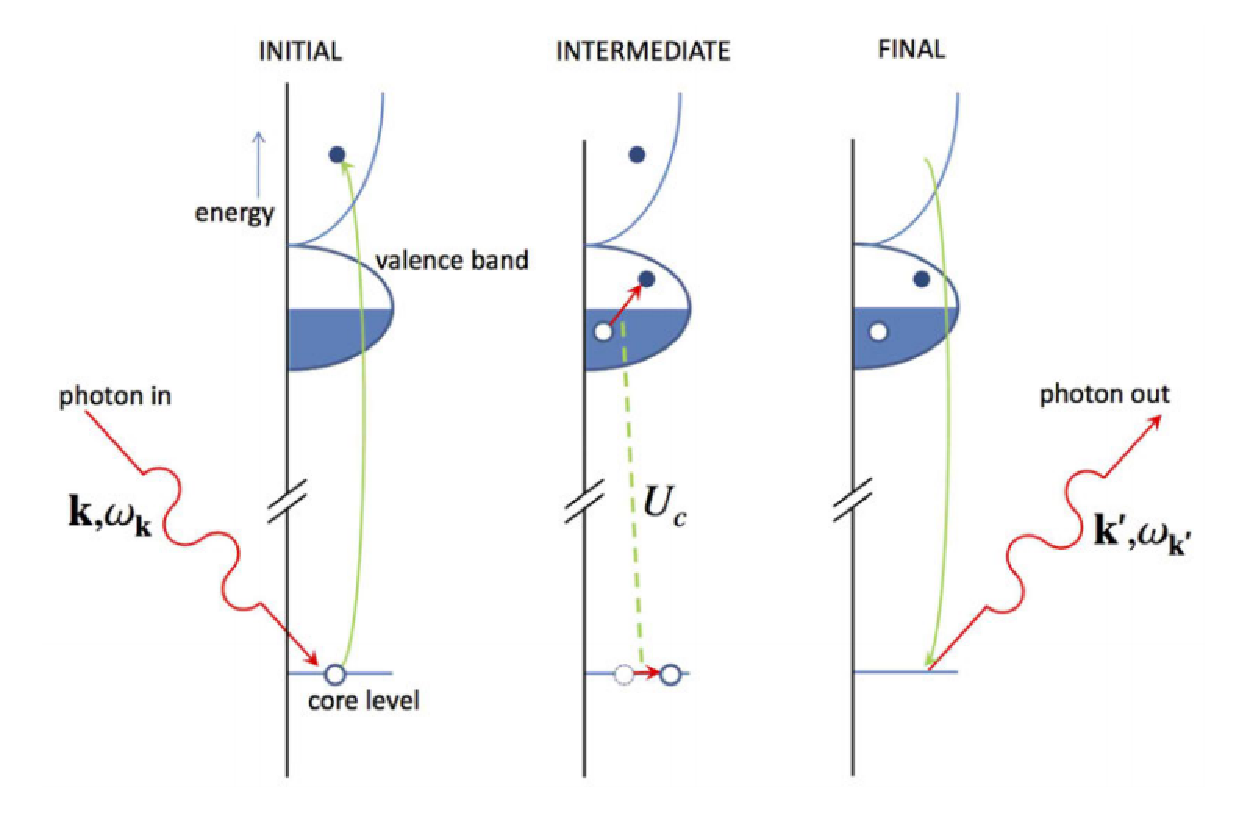
\includegraphics[width=0.8\columnwidth, height = 5 cm]{RIXSprocess.pdf}
\caption{Typical indirect RIXS process involving creation of a hole in the valence shell due to strong core hole-electron coulomb interaction \cite{GuarisePhD} (Picture taken from \cite{GuarisePhD})}
\label{Process} 
\end{figure}
\indent As is seen in \ref{Process} the RIXS process can be decomposed in X-ray Absorption (XAS) and X-ray photoemission (XPS or XES) with some intermediate interaction for the indirect RIXS. As far as XAS is well understood, it isn't the same case for XPS. Without any polarization analyzer for the scattered beam we can only measure the intensity of the scattered wave (the number of photons per second at the detector), which results in difficulties to analyse RIXS spectra. Properly guessing the polarization of the scattered wave rises the possibilty to investigate magnetic properties of the material in terms of magnon disperision. Nevertheless even with symmetry arguments it remains unclear how to determine the polarization in a re-excitation process (of a photon). 
%
%\iffalse %Commented section - is not compiled
The averaging techique mentioned in the introduction, would for the general polarization vector:
\begin{equation}
\vec{e}_{out}=a\vec{e}_{LV}+\sqrt{1-a^2}e^{i\phi}\vec{e}_{LH},
\end{equation}
\noindent where the polarization was decomposed in the base of linear polarizations (for $a=\frac{1}{\sqrt{2}}$ and $\phi=\pm\frac{\pi}{2}$ we have circular polarization); take the form:
%
\begin{equation}
I_{RIXS}\varpropto\int_0^1 da\int_0^{2\pi} d\phi f(a,\phi)\left|\vec{e}_{out}^*(a,\phi)\omega\tensor{\sigma}\vec{e}_{in}\right|, 
\end{equation}
\noindent with $f(a,\phi)$ being the weighting factor. In the case of direct and elastic scattering one can assume that linear polarization remains linear (with every possible rotation) and circular polarization remains circular. This would mean the weighting function must be slowly varying (and smoothly) with the angle $\phi$ or even set to be independent to that angle. The resulting integral would be angle independent and yielding only a multiplication by $2\pi$.As for the normalization factor $a$ there can't be made an assumption like the on above. Moreover the dependence of the weighting factor to the $a$ value is . . . . . none.
%\fi %Til this point
%
%-----------------------------------EXPERIMENTAL-----------------------------------------------------
\section{EXPERIMENT}
The experiment was done at the Lawrence Berkeley National Laboratory using synchrotron radiation generated by an undulator. The experiment was repeated for various energy values in the range $925-980$ $eV$ and each one was measured between constant k-points (so the peak would be in the middle of the range). It was taken into account that the beamline itsef changes the incoming polarization (by a set of imperfect mirrors and measplitters), so the polarization was appropriately changed to have the desired incident polarization.
\begin{figure}[h]
	
\includegraphics[width = 0.5\columnwidth, height = 2.5 cm]{hmm.jpg}
\end{figure}
%----------------------------------------RESULTS-------------------------------------------------------
%
%----------------------RIXS spectra-----------------------------------
\begin{figure*}
	\begin{minipage}[bh!]{\columnwidth}
		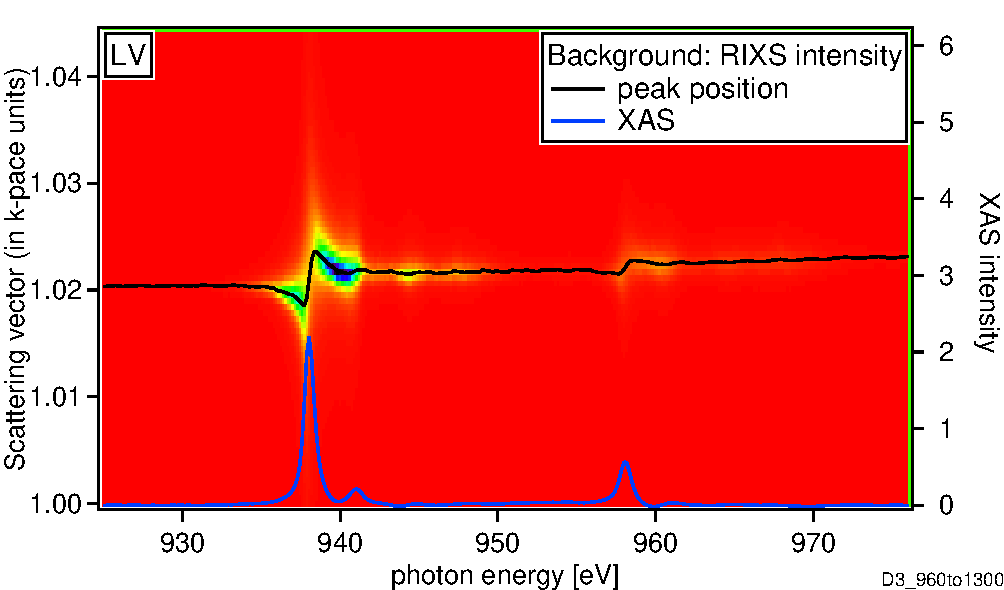
\includegraphics[width = \textwidth, height = 3.6 cm]{./RIXS/LV(960).pdf}
	\end{minipage}
	\hfill
	\begin{minipage}[bh!]{\columnwidth}
		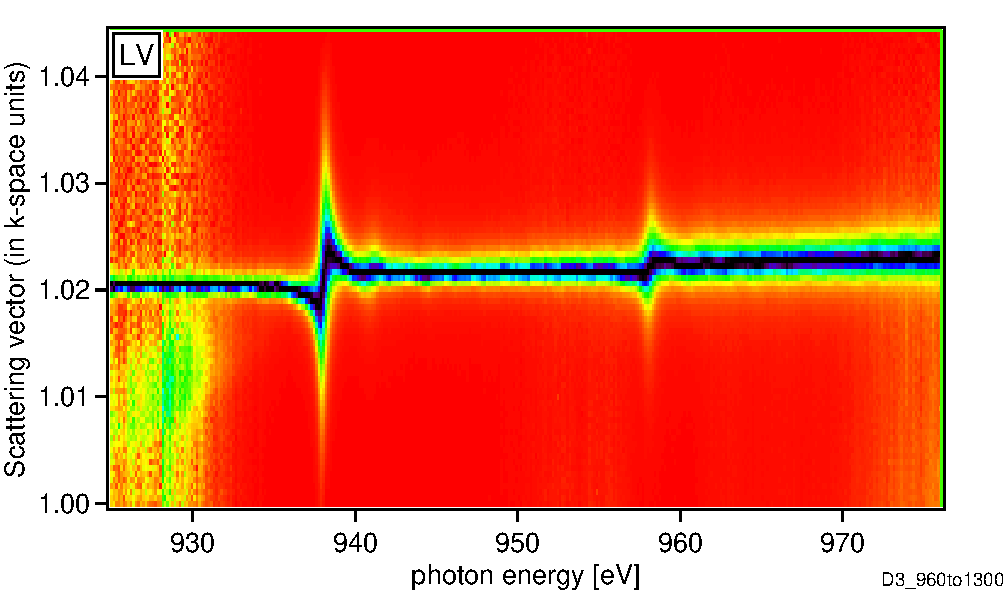
\includegraphics[width = \textwidth, height = 3.6 cm]{./RIXS/LV(960)norm.pdf}
	\end{minipage}
	\caption{(Left) Results of RIXS for s polarization as a intensity map (background). The black curve is the bragg peak position (left axis) for each energy, whereas the blue one is the    X-ray Absorption intensity (right axis)\\  
\noindent (Right) RIXS intensity normalized along the x-axis}
	\label{RIXS_LV}
\end{figure*}
%----------RIXS--------------
\begin{figure}
	\begin{minipage}[tp]{0.45\columnwidth}
		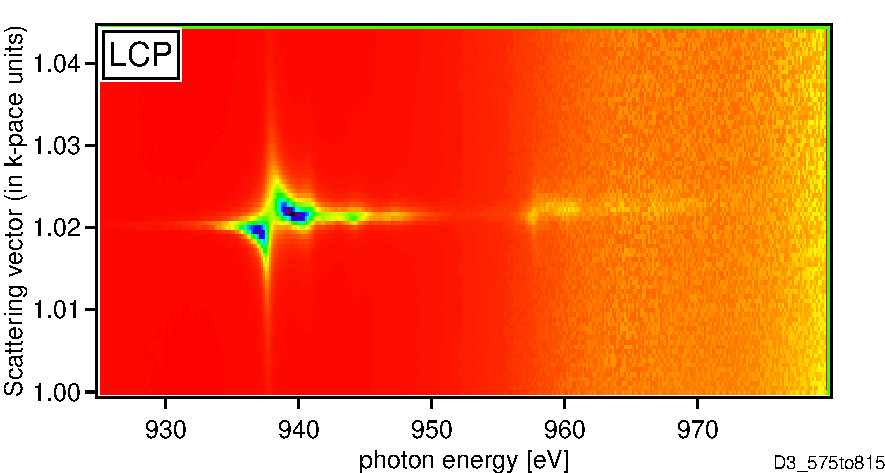
\includegraphics[width = \textwidth, height = 2.8cm]{./RIXS/LCP.pdf}
	\end{minipage}
	\begin{minipage}[tp]{0.45\columnwidth}
		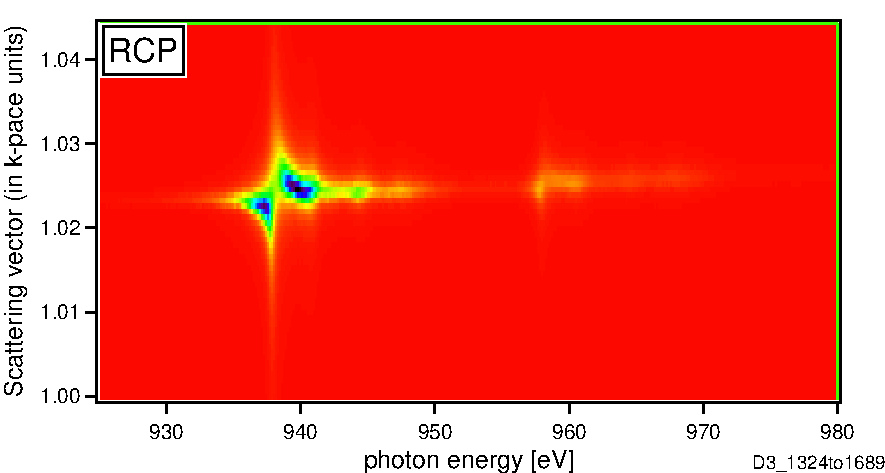
\includegraphics[width = \textwidth, height = 2.8cm]{./RIXS/RCP.pdf}
	\end{minipage}
	\begin{minipage}[tp]{0.45\columnwidth}
		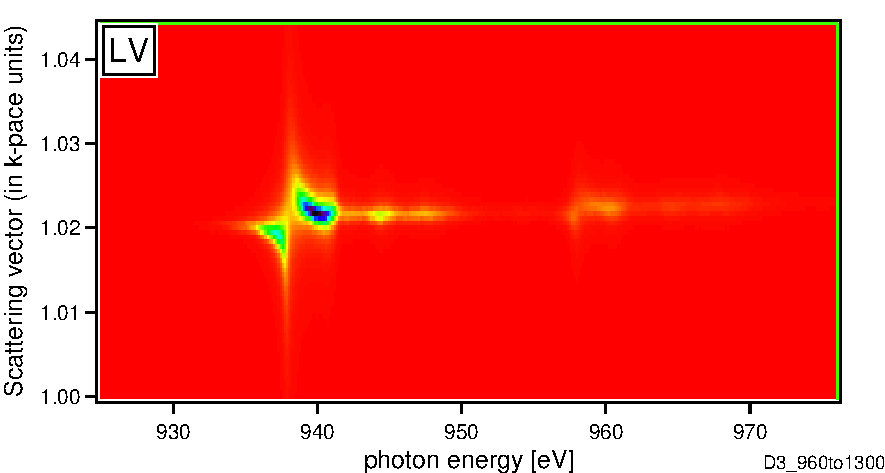
\includegraphics[width = \textwidth, height = 2.8cm]{./RIXS/LV.pdf}
	\end{minipage}
	\begin{minipage}[tp]{0.45\columnwidth}
		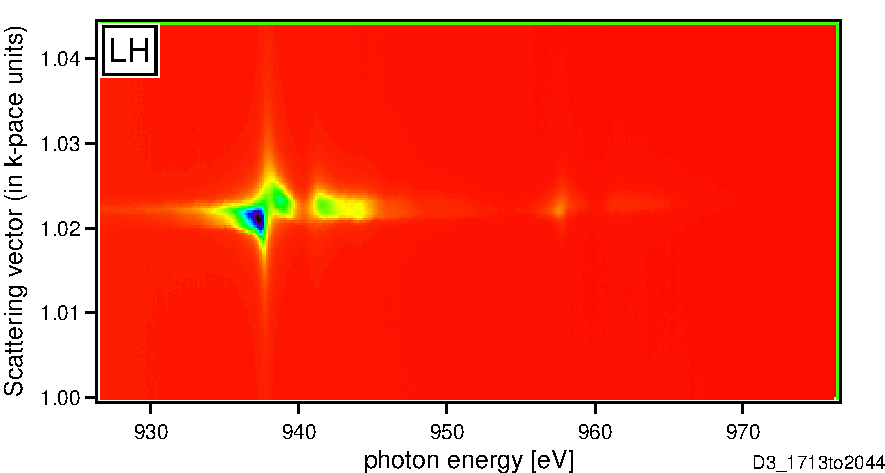
\includegraphics[width = \textwidth, height = 2.8cm]{./RIXS/LH.pdf}
	\end{minipage}
	\begin{minipage}[tp]{0.45\columnwidth}
		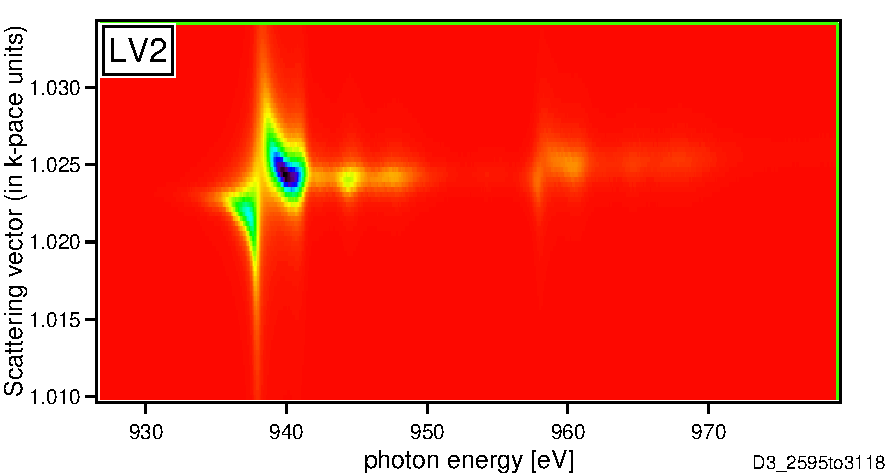
\includegraphics[width = \textwidth, height = 2.8cm]{./RIXS/LV2.pdf}
	\end{minipage}
	\begin{minipage}[tp]{0.45\columnwidth}
		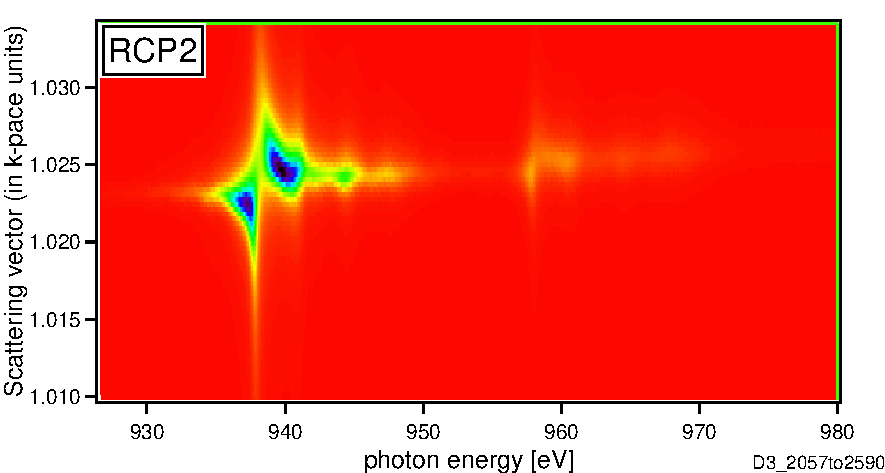
\includegraphics[width = \textwidth, height = 2.8cm]{./RIXS/RCP2.pdf}
	\end{minipage}
	\label{RIXSall}
	\caption{RIXS spectra as intensity map for different polarization: s- (Middle-left and Bottom-left), p- (Middle-right), left circular (Top-left) and right circular polarization (Top-right and Bottom-right)}
	\begin{minipage}[tp]{0.45\columnwidth}
		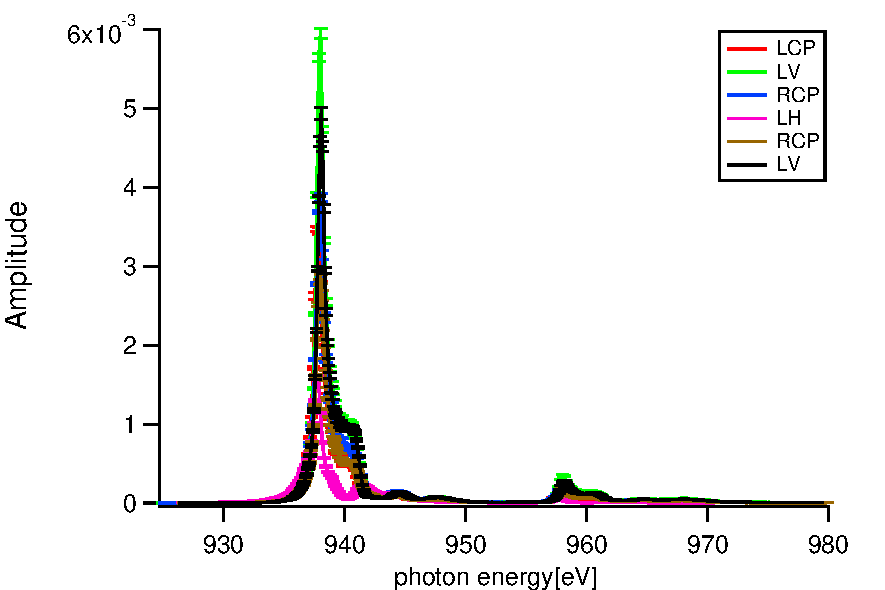
\includegraphics[width = \textwidth, height = 2.7cm]{amplitude.pdf}
	\end{minipage}
	\begin{minipage}[tp]{0.45\columnwidth}
		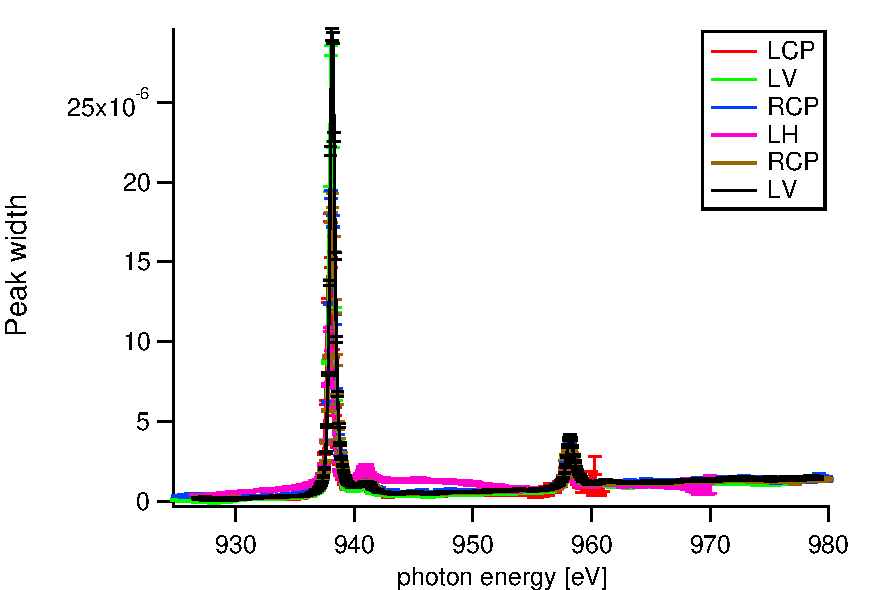
\includegraphics[width = \textwidth, height = 2.7cm]{width.pdf}
	\end{minipage}
	\begin{minipage}[tp]{0.45\columnwidth}
		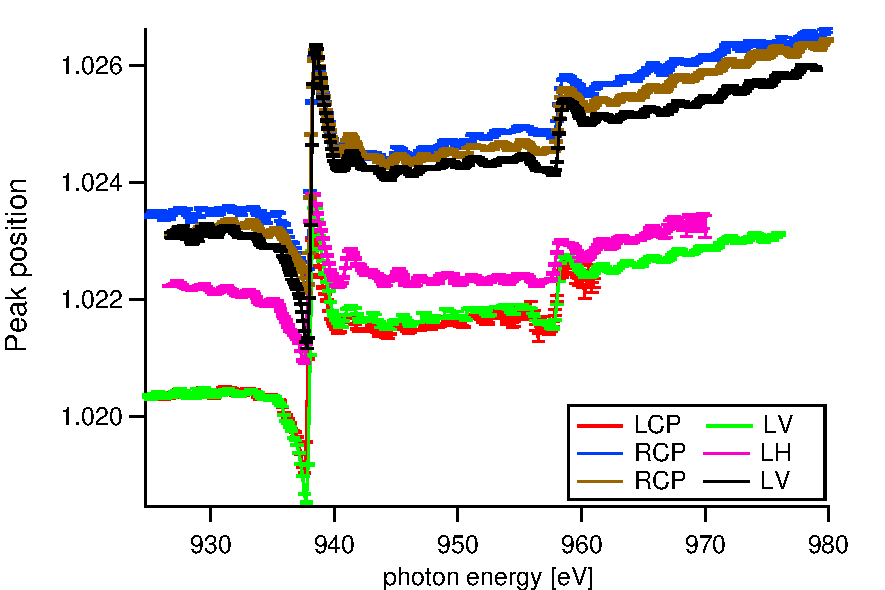
\includegraphics[width = \textwidth, height = 2.7cm]{position.pdf}
	\end{minipage}
	\begin{minipage}[tp]{0.45\columnwidth}
		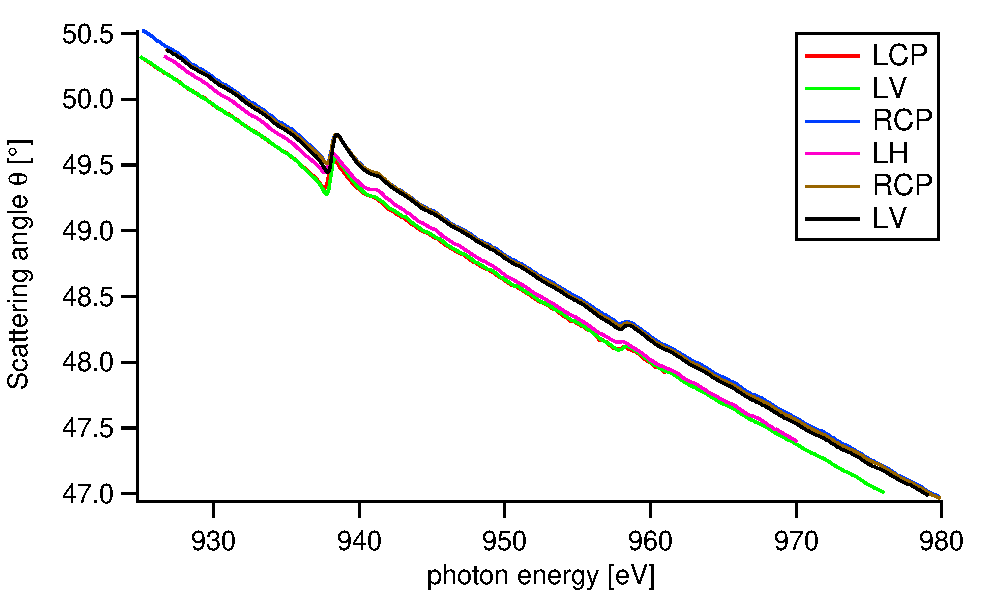
\includegraphics[width = \textwidth, height = 2.7cm]{ScatAng.pdf}
	\end{minipage}
	\label{FitResults}
\caption{Fit results of RIXS spectra (\ref{RIXS_LV},\ref{RIXSall}) using a Lorentzian lineshape resulting in quantities like: Amplitude (Top-left), peak width (Top-right) and peak position (Bottom-left). Using the Bragg condition we immeadetly obtain the scattering anlge $\theta$ from the peak posiition (bottom-right)}
\end{figure}
%
\section{RESULTS}
\subsection{RIXS spectra}
Measurments on the copper $L_{2,3}$ edge gives detailed information on the optical properties in the material. In this system there can only be dipole excitation as quadrupole excitation is fobidden by symmetry and higher terms are typically to weak. Thus only dipole, dd and magnon excitations are seen in the data. The results shown in \ref{RIXS_LV} for LV (s) polarization exhibits a strong intensity peak at the copper L edges. We observed the same beaviour for differend kinds of polarization, shown in \ref{RIXSall}. The first plot has strong deviations in intensity above the $L_2$ edge, which is possibly resulting in bad measurment for those energies. The middle plots presents the most important feature in this paper, namely the magnetic ordering in the sample. We see directly an anisotropy in linear polarization due to linear dichroism effect, which is strong in antiferromagnets. 
For circular polarization the difference is much lower, thus ferromagnetic ordering can be excluded (circular dichroism is strong in ferromagnets). The importance of this effect lies within symmetry conisderation of the optical conductivity (see appendix C). In magnetic materials this tensor becomes antisymmetric in his offdiagonal elements, which is significant for further analysis in the next section.\\
\indent For each energy the RIXS spectrum (along the different q-values) has a Lorentzian shape. This means we can fit the RIXS spectrum with a lorentzian curve. The spectrum was fitted in the Igor 6.37 software using the Lorentzian $y=y_0+\frac{ A}{(x-x_0)^2+B}$, whose FWHM equals $2\sqrt{B}$ and the results are shown in the \ref{FitResults}. We immeadetly notice the resonant behaiour of peak position with a shape similiar to the real part of the refractive index. Therefore one can assume there exists a direct mapping of the peak position to thee refractive index. Making use of Bragg's law one can derive the following equation for the deviation of the real part of the refractive index \cite{Seve}:
\begin{equation}\label{RefRe}
\delta\left(E\right)=\frac{1}{2}\sin^2\theta\left(E\right)-\left(\frac{hc}{2dE}\right)^2,
\end{equation}
\noindent with $d$ being the lattice constant in the (001) direction and $\theta$ the scattering angle. The scattering angle can be obtained from the peak position by the formula \ref{eq: ScatAngle} (see appendix B), which is obtained through the bragg condition. the data in \ref{RIXS_LV} on the right plot exhibits an increase in the FWHM of the lorentzian curve, which then relates to the linear absorption coefficients. On the other hand the linear absorption coefficient is directly related to the imaginary part of the refractive index by 
$\mu=\frac{2\omega\kappa}{c}$. As was proved by Seve \cite{Seve} the FWHM of these lorentzians equals to $\frac{\mu}{\sin\theta}$, which then yields the formula:
\begin{equation}\label{RefIm}
\kappa=\left(\frac{hc}{2dE}\right)^2\sqrt{B(E)}x_0(E),
\end{equation}
\noindent where $B$ is denoted as the peak width and $x_0$ is the bragg peak position.  Applying the formulas above (\ref{RefRe} and \ref{RefIm}) yields the complex refractive index presented in \ref{Refractive}. We notice the similiarity of the imaginary part of the refractive index (except for the LH polarization), which is not the case for the real part. 

%----------Refractive-----------------
\begin{figure}
	\begin{minipage}[t]{0.9\columnwidth}
		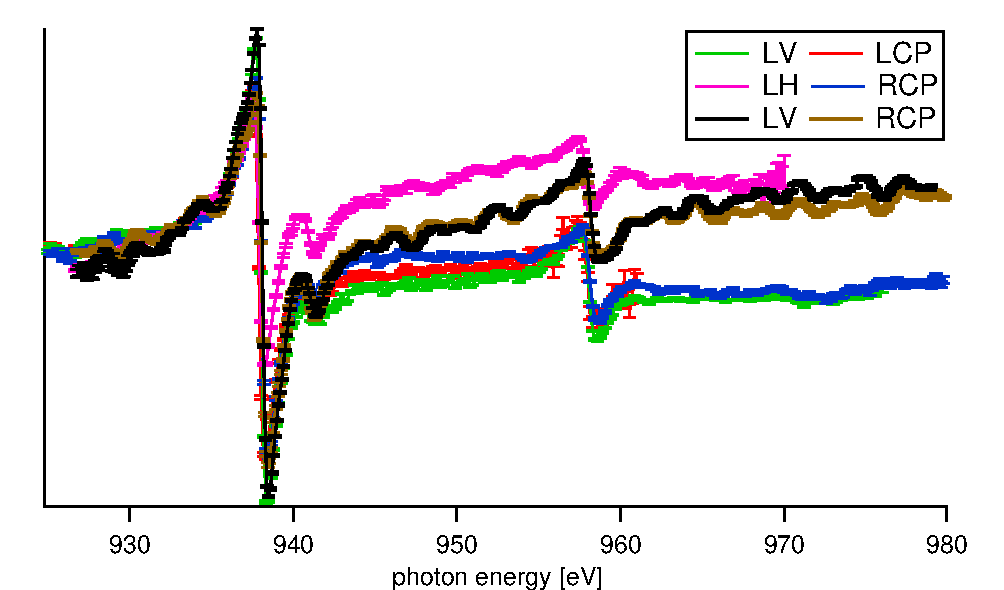
\includegraphics[width = \textwidth, height = 3cm]{RefIndRe.pdf}
	\end{minipage}
	\begin{minipage}[t]{0.9\columnwidth}
		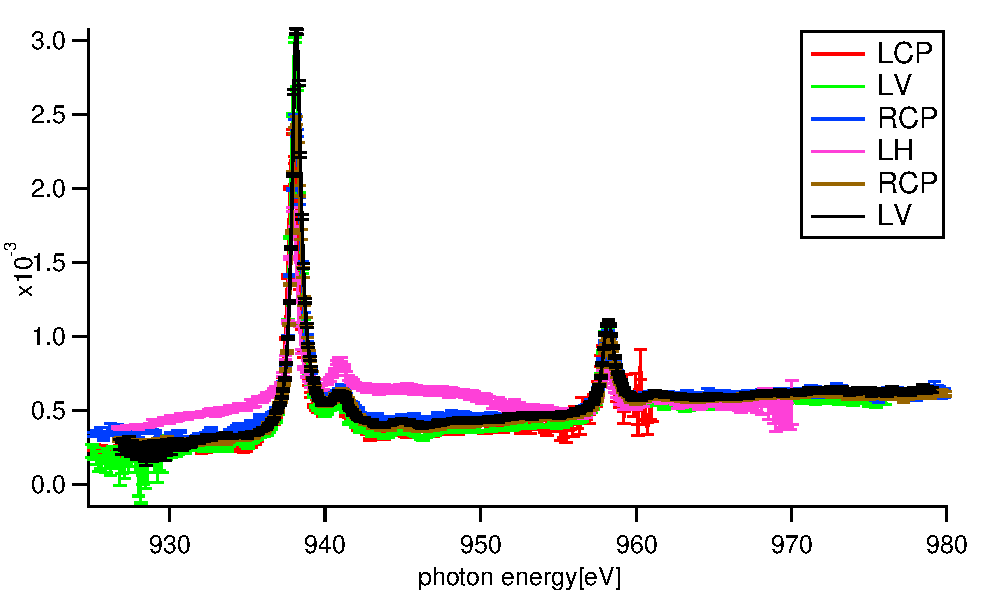
\includegraphics[width = \textwidth, height = 3cm]{RefIndIm.pdf}
	\end{minipage}
	\label{Refractive}
\caption{Complex refractive iondex for different polarizations: (top) real part and (bottom) imaginary part.}
\end{figure}
%
%----------------------XAS spectra-----------------------------------
\subsection{X-ray Absorption Spectroscopy}
As mentioned before RIXS can be essentially seperated into x-ray absorption (XAS) and x-ray photoemission spectroscopy (XPS) with some intermediate interaction (for indirect RIXS) described by the green's function of the Kramers-Heisenberg Hamiltonian \cite{GuarisePhD}. The XAS spectrum is directly proprtional to the absorption of the crystal which gives information on magnetic properties of the material. The difference in the absorption using left- and right-cirular polarized x-rays in called circular magnetic x-ray dichroism (CMXD) ( the similiar differnec in linear polarized light is called LMXD). In order to obtain the CMXD one needs to preserve only the relevant resonances at the copper $L_3$ and $L_2$ edges, which means one needs to model and substract the background assossiated with the excitation of the core electrons into the continuum. The way to do so is to use user-defined bakground function (using for example the arcus tangent) or using the shirley algorithm \cite{Gomez,Shirley}, this is shown in the \ref{TEY}(top graph).
One directly notice that the Shirley algorithm is fitting the backgound much better. This method was used for different polarizations and the corresponing aborption spectra are drawn in \ref{TEY} (bottom graph). Now one can proceed to evaluate the CMXD and LMXD on the copper L edges.\\
%
\begin{figure}
    \begin{minipage}[t]{\columnwidth}
        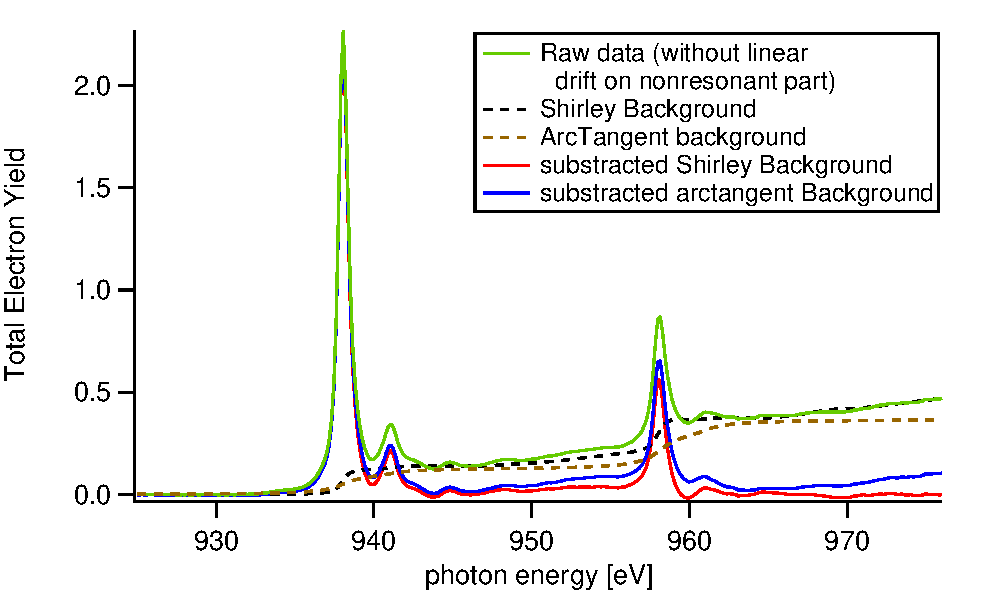
\includegraphics[width=0.9\textwidth, height=3.5cm ]{ShirleyBack.pdf}
    \end{minipage}
    \hfill
	\begin{minipage}[t]{\columnwidth}
        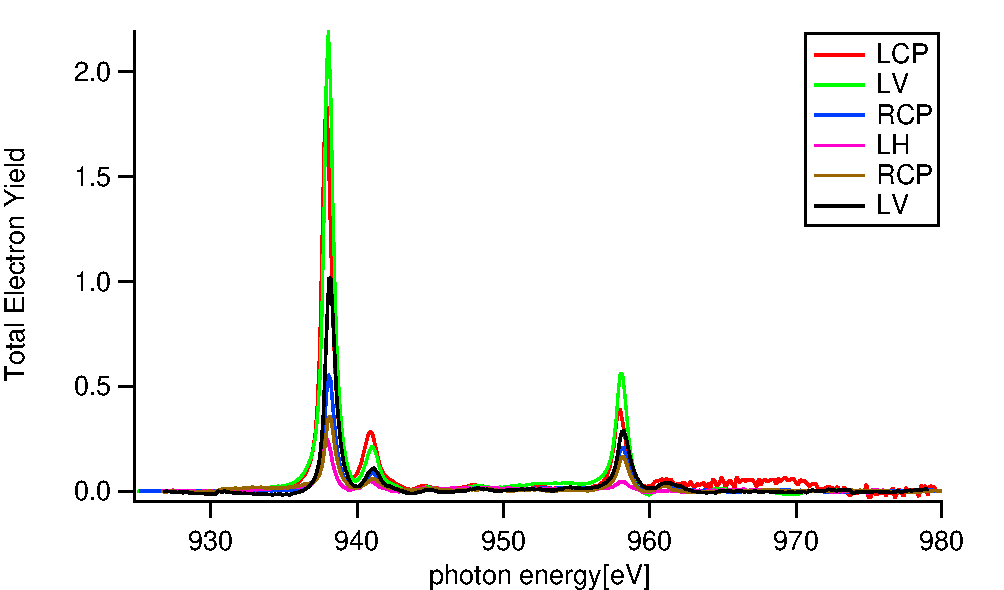
\includegraphics[width=0.9\textwidth, height=3.5cm]{TEY.pdf}
    \end{minipage}
\caption{Absorption spectra and modelled background with two different methods (top) and Absorption spectra with substracted shirley backgound (bottom)}
\label{TEY}
\end{figure}
%
\indent  Not only gives the absorption spectra detailed information about dichroic effects, but also it rises the oppportunity to calculate the optical conductivity tensor \cite{Haverkort}. The relation linking the absorption cross section to the conductivity tensor is as follows \cite{Ament2018}:
%
\begin{equation}
I_{XAS}(\omega)= -\frac{1}{\pi} \Im(\vec{e}^*\tensor{\sigma}(\omega)\vec{e}),
\end{equation}
%
with $\vec{e}$ being the incoming polarization. The forcmula above is directly obtained by the optical theorem \cite{Newton}. the optical theorem links the imaginary part of the scattering amplitude (related to the conductivity) to the absorption cross section (direlty proportional to the TEY and thus essentially what we measure in XAS). Using this relation above and the optical conductivity tensor derived in appendix C (equation \ref{eq:OptCond}) we obtain a system of equations of the form (in matrix notation):
\begin{widetext}
\begin{equation}
\left(\begin{array}{c}
I_{LV} \\ I_{LH} \\ I_{LCP} \\ I_{RCP}
\end{array}\right)=-\frac{1}{\pi}\left(
\begin{array}{cccc}
1&0&0&0\\
\sin^2\theta&0&0&\cos^2\theta\\
\frac{1+\sin^2\theta}{2}&m_z\sin\theta&-m_y\cos\theta&\frac{\cos^2\theta}{2}\\
\frac{1+\sin^2\theta}{2}&-m_z\sin\theta&m_y\cos\theta&\frac{\cos^2\theta}{2}\\
\end{array}\right)\left(
\begin{array}{c}
\Im\sigma_{xx}\\ \Re\sigma_{xy}\\ \Re\sigma_{xz}\\ \Im\sigma_{zz}
\end{array}\right),
\end{equation}
\end{widetext}
\noindent where on the left side we have the XAS intensities for different polarizations. Inversing this matrix equation yields the desired result for the tensor elements. However we only obtain the imaginary part in the diagonal and the ral part for the offdiagonal elements. Their corresponding complex companion was calculated by the Kramers-Kronig transforms (see next section) and the resulting tensor elements are show in \ref{OpticalCond} (left). By direct comparison with theoretical calculations \cite{Haverkort} we see equivalence for the $\sigma_{xx}$ element (and thus also $\sigma_{yy}$). However the $\sigma_{zz}$ vanishes in the theoretical consideration due tu the ground state symmetry. the calculations made above doesn't consider this symmetry and thus the result is something artificial from the calculations; it can only be excluded in the use of symmetry argruments. Having a look at the offdiagonal elemetns we notice agreement with Haverkorts's results \cite{Haverkort} in the $L_3$ edge, but not for the $L_2$ edge (it is not inverted). The reason might be also artificial in the calculations and thus only obtainable in symmetry considerations.\\
\indent One can directly relate these results to calculate the dielectric permittivity tensor (formula \ref{DielOpt}, see appendix C), shows in \ref{OpticalCond} (right). Furthermore the dielectric tensor yields more possibilities in material analysis. The kernel of this tensor can be viewed as the polarization of the waves propagating in the medium, which are allowed by the crystal symmetry \cite{Starke}. The kernel can be calculated by the simple formula:
\begin{equation}
\tensor{\varepsilon}(\omega,\vec{k})\vec{e}(\omega,\vec{k})=0,
\end{equation}
\noindent where we no longer can assume the wavevector-independent form of the dielectric tensor. Therefore in our case it won't be possible to calculate those polarizations.
%
\begin{figure*}
	\begin{minipage}[b]{0.95\columnwidth}
		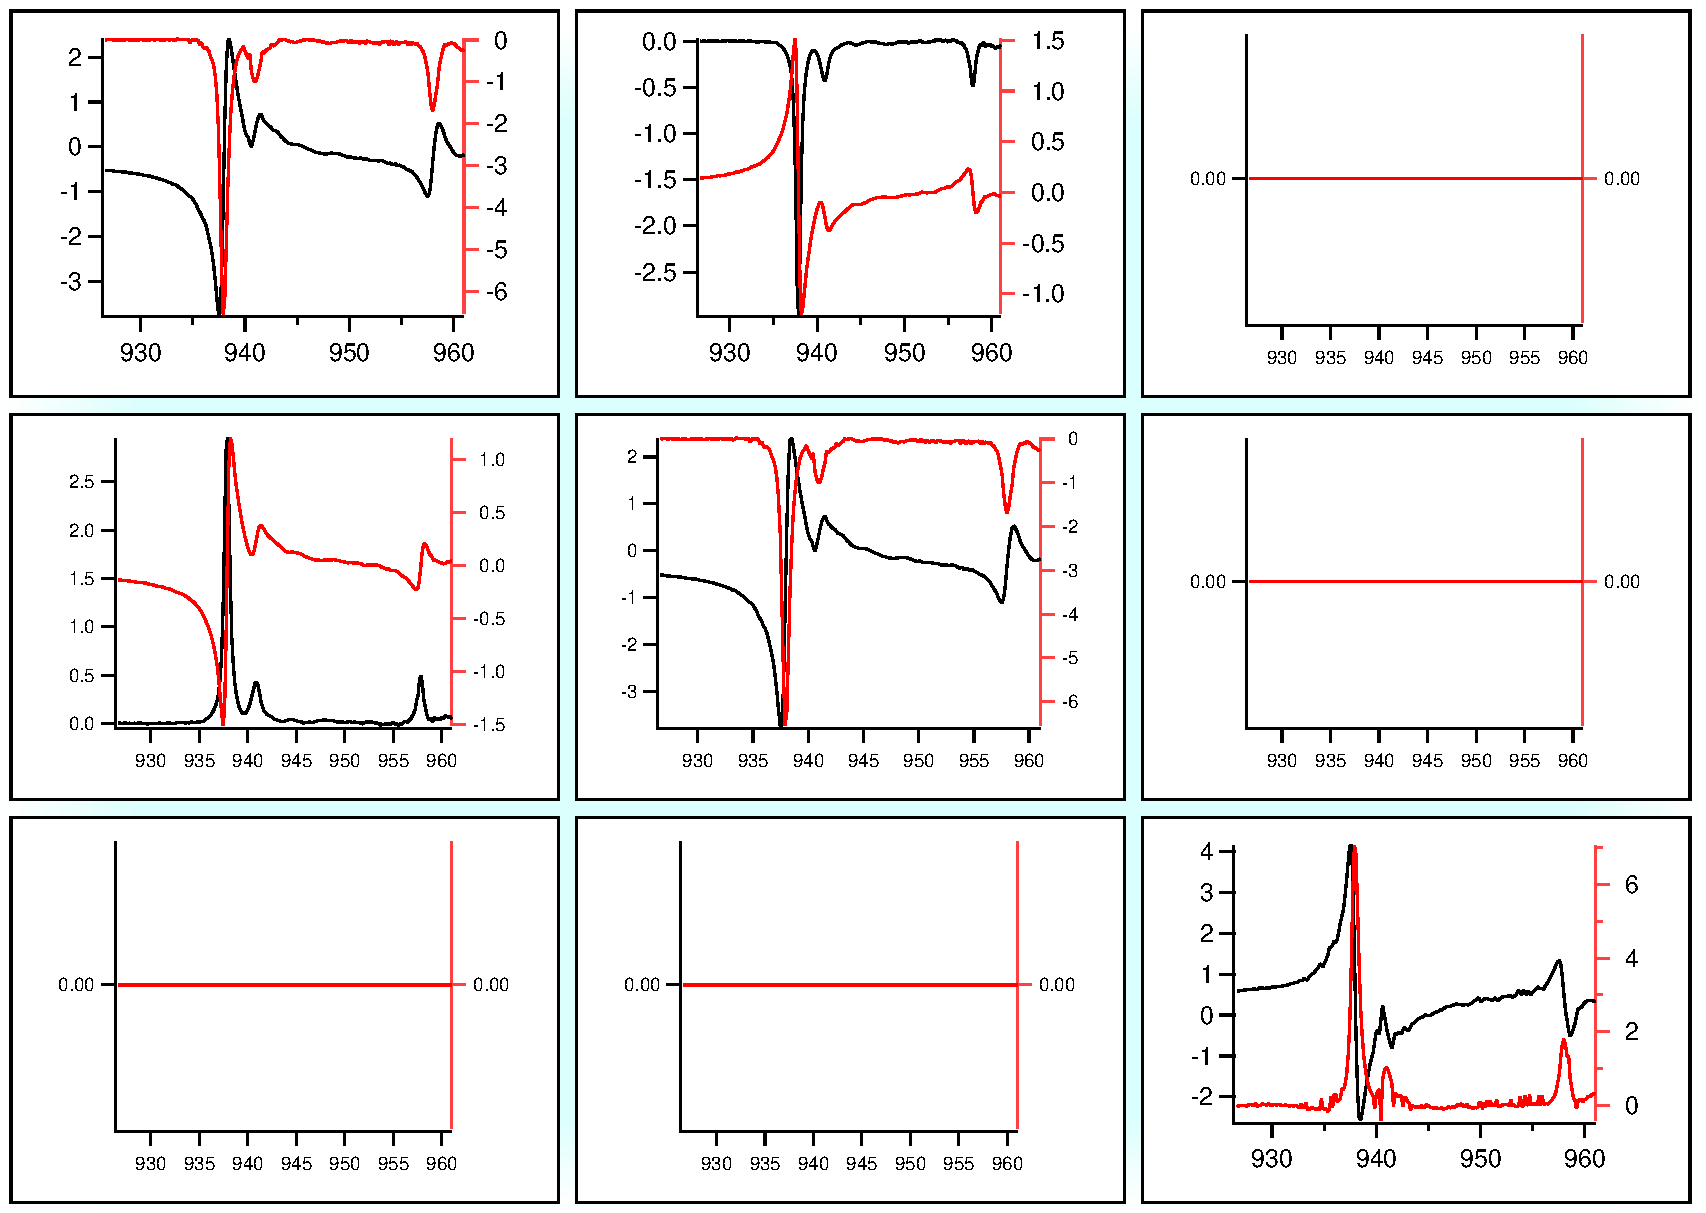
\includegraphics[width = \textwidth, height = 7cm]{OptCond.pdf}
	\end{minipage}
	\hspace{8mm}
	\begin{minipage}[b]{0.95\columnwidth}
		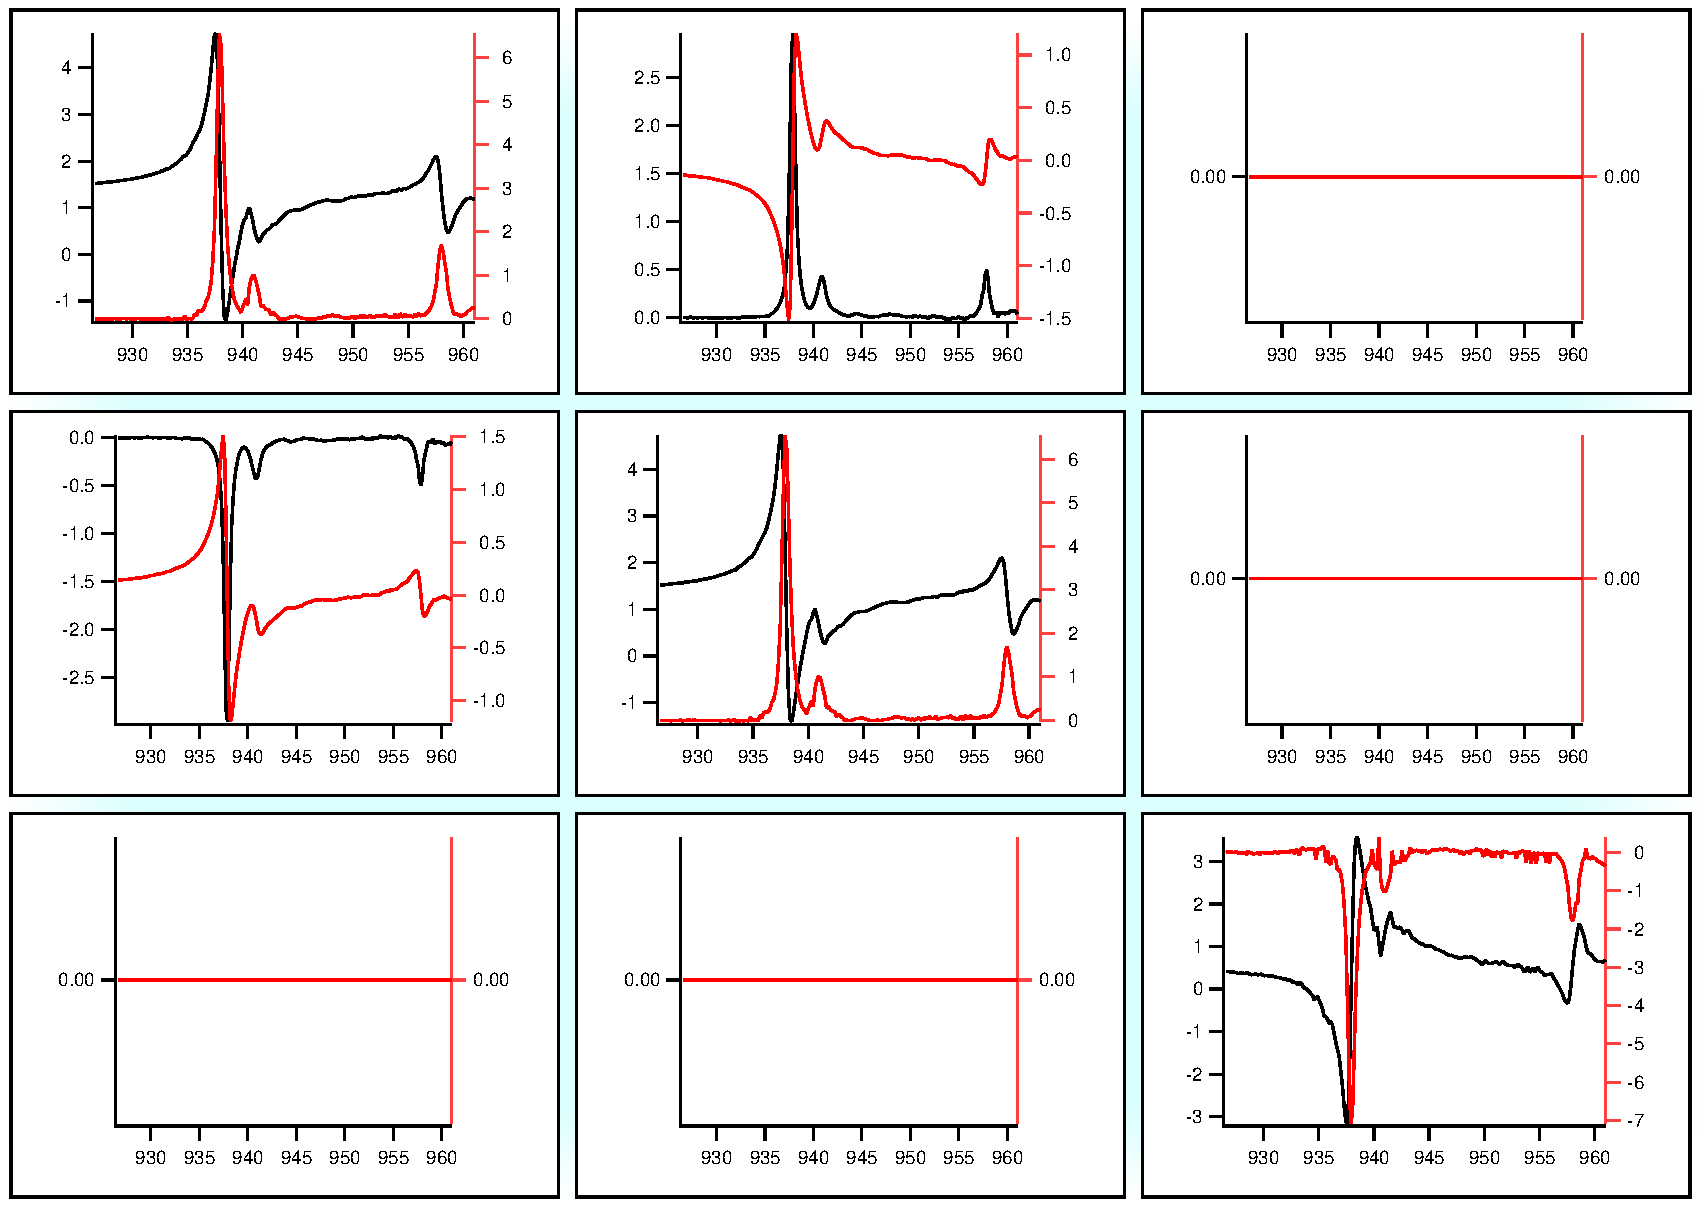
\includegraphics[width = \textwidth, height = 7cm]{DielTens.pdf}
	\end {minipage}
	\caption{\label{OpticalCond} (Left) The resulting optical conductivity tensor (each subplot represents the corresponding tensor element, left top is $\sigma_{xx}$ and so on). The black curves are the real parts of the tensor elements (with the left axis) and the red ones are the imaginary parts (with the right axis). (Right) The relative dielectric permittivity tensor with same same distribution and labeling as the optical conductivity tensor. The bottom axis is in each case the photon energy in $eV$.}
\end{figure*}
%
%-----------------------------------------------------Kramers-Kronig---------------------------------
\section{KRAMERS-KROING ANALYSIS}
The results from the RIXS experiments allows one to investigate their consistnecy within the Kramers-Kronig (KK) analysis. The KK relations are obtained from the Hilbert transform for complex responce functions \cite{Lucarini}. Thos responce functions must fullfil several properties, mainly: being analytic in the complex upper half plane, they must fullfil the principle of causality, which states $G(t)=0$ for $t<0$ for any response function $G(t)$ and sufficient asymptotic behaviour for large $\omega$. Only function, which fullful these conditions can be related y the Hilbert transform and thus the KK relation holds. The usual KK relations for an responce function $G(\omega )$ are as follows \cite{Lucarini}:
	\begin{equation} %General Kramers Kronig
	\Re G(\omega)=\frac{1}{\pi}\wp\int_{-\infty}^{\infty}d\omega'\frac{\Im G(\omega')}{\omega'-\omega}
	\end{equation}
	\begin{equation}
	\Im G(\omega)=-\frac{1}{\pi}\wp\int_{-\infty}^{\infty}d\omega'\frac{\Re G(\omega')}{\omega'-\omega},
	\end{equation}
\noindent where $\wp$ denotes the cauchy principal value for integration of a function with singularities (poles). For the refractive index $n_c=1-\delta+i\kappa=n+i\kappa$ these relations can be modified through the property: $n(-\omega)=n(\omega)$, which yields the relations:
	\begin{equation}% Kramers Kronig for refractive index
	n(\omega)-1=\frac{2}{\pi}\wp\int_{0}^{\infty}d\omega'\frac{\omega' \kappa(\omega')}{\omega'^2-\omega^2}
	\end{equation}
	\begin{equation}
	\kappa(\omega)=-\frac{2\omega}{\pi}\wp\int_{0}^{\infty}d\omega'\frac{ n(\omega')-1}{\omega'^2-\omega^2}\\ \\
	\end{equation}
Similiarly the dielectric function has this relation (all tensor elements independently), but the optical conductivity (for each tensor element) has similiar relations, namely:
	\begin{equation}% Kramers Kronig for optical conductivity
		\Re\sigma(\omega)=\frac{2}{\pi}\wp\int_{0}^{\infty}d\omega'\frac{\omega' \Im\sigma(\omega')}{\omega'^2-\omega^2}
	\end{equation}
	\begin{equation}
		\Im\sigma(\omega)=-\frac{2\omega}{\pi}\wp\int_{0}^{\infty}d\omega'\frac{\Re\sigma(\omega')}{\omega'^2-\omega^2}\\
	\end{equation}
\indent The KK transform (KKT) requires an infinite frequency range, which is experimentally impossible. The finite energy range results mostly in problem using the KKT, especially on the boundaries of the frequency range. Different approaches are made \cite{Johnson, Kuzmenko, Emeis, Llosa} to improve this strong tool in optical measurments. Whether using Fourier Transform (FT) \cite{Johnson} or extrapolating the data outside the measured region \cite{Emeis} we see significant improvment in this optical tool. Without any improvements the KKT shows strong "edge effects" as show in the left side of \ref{KKT}. Even if one could use the simple KKT on finite range for obtaining the real part; it is not so obvious for the imaginary part, because of the strong "edge effects". In comparison on the right side of \ref{KKT} we see much better equivalence of the KKT results and the measured data using similiar extrapolation as in \cite{Emeis}, but the data was set to saturate beyond the measured region. 
%-----------KKT--------------
\begin{figure}
	\begin{minipage}[t]{0.45\columnwidth}
		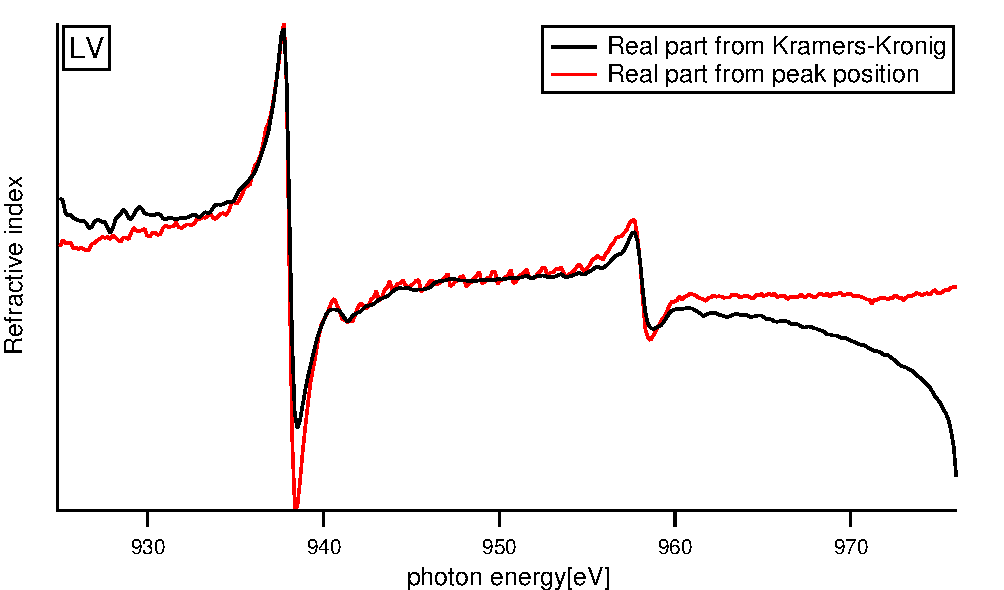
\includegraphics[width=\textwidth,height=2.5cm]{./KKT/KKreLV_edge.pdf}
	\end{minipage}
	\begin{minipage}[t]{0.45\columnwidth}
		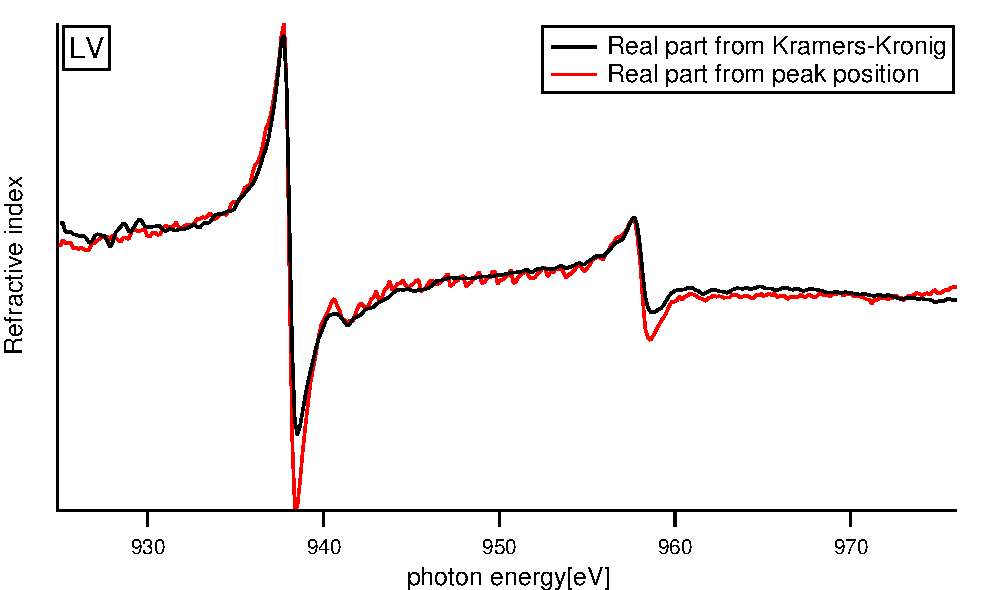
\includegraphics[width=\textwidth,height=2.5cm]{./KKT/KKreLV.pdf}
	\end{minipage}
	\begin{minipage}[t]{0.45\columnwidth}
		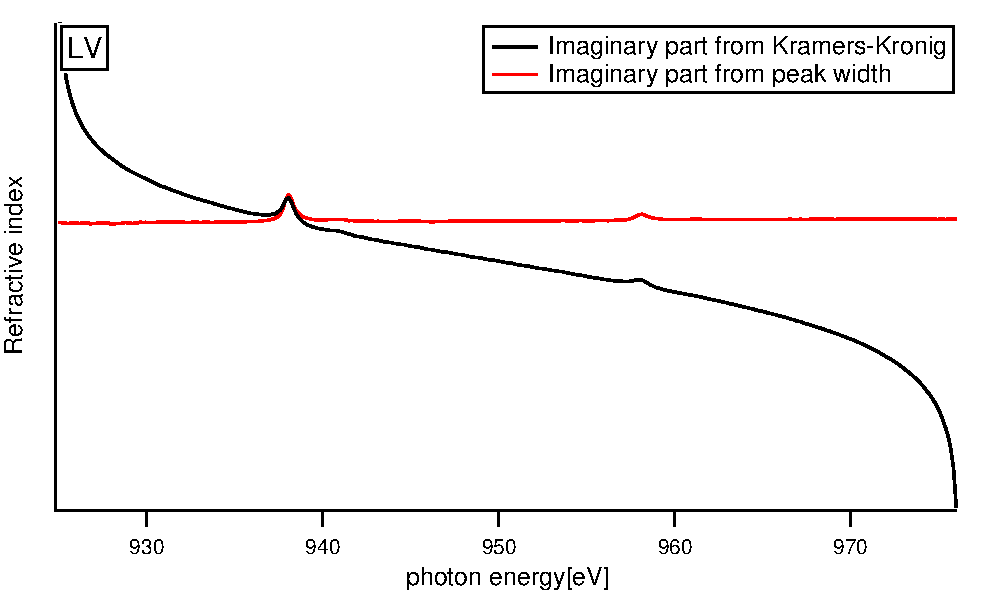
\includegraphics[width=\textwidth,height=2.5cm]{./KKT/KKimLV_edge.pdf}
	\end{minipage}
	\begin{minipage}[t]{0.45\columnwidth}
		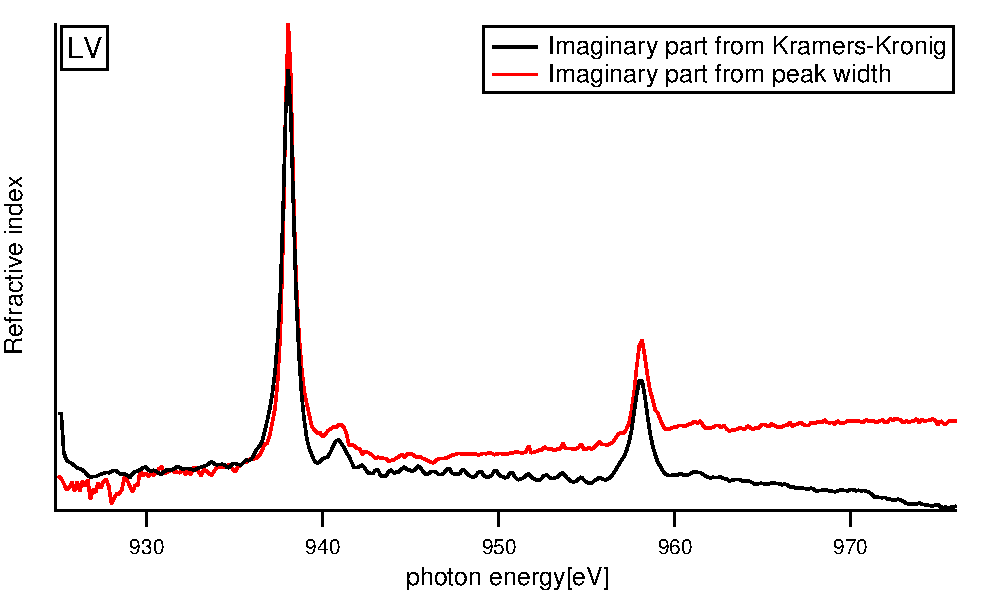
\includegraphics[width=\textwidth,height=2.5cm]{./KKT/KKimLV.pdf}
	\end{minipage}
	\caption{\label{KKT} Kramers-Kronig transforms of complex refractive index for LV polarization for finite energy range (left panels) and using data extrapolaton on the boundaries (right panels)}
\end{figure}
%
%-----------------------------------------------------SUMMARY---------------------------------
\section{SUMMARY}
%
%
%
%
%---------------------------------------------------------------------------------------------------
%-----------------------------------------------------APPENDIX---------------------------------
%---------------------------------------------------------------------------------------------------
\appendix
%----------------------------------------POLARIZATION-------------------------------------------------------
\section{Polarization}
\renewcommand{\thefigure}{Fig.A\arabic{figure}}
\renewcommand{\theequation}{Eq.A\arabic{equation}}

Choosing the coordinate system can be complicated in more complex systems. We would like to choose the coordinate system to coincide with the crystal ones, which means we have to construct properly the polarization vector of the incident wave. To do so we need to define various parameters. In order to simplify we let the coodinate system be defined with the scattering plane in the yz plane. This means we only need the scattering angle to define the polarization as is shown in \ref{polarization}. One can describe the palarization vector using rotation matrices, namely:
\begin{equation}
\begin{split}
\vec{e}_{in} = \left(
\begin{array}{ccc}
1&0&0\\
0&\cos\varphi&-\sin\varphi\\
0&\sin\varphi&\cos\varphi\\
\end{array}\right)\\
\times\left(
\begin{array}{ccc}
\cos\xi&\sin\xi&0\\
-\sin\xi&\cos\xi&0\\
0&0&1
\end{array}\right)\left(
\begin{array}{c}
1\\0\\0
\end{array}\right)=\\
=\left(
\begin{array}{c}
\cos\xi\\ \cos\varphi \sin\xi\\ \sin\varphi \sin\xi
\end{array}\right),
\end{split}
\end{equation}
\noindent which consists of a rotation around the $z-axis$ with an angle $\xi$ to distinguish types of polarization and a rotation around the $x-axis$, where $\varphi$ denotes the angle between the incident beam and the scattering vector. The angle $\xi$ takes the value $\xi=0$ for s-type polarization (out of plane: LV-left vertical) and $\xi=\frac{\pi}{2}$ for p-polarization (in scattering plane: LH-left horizontal). The polarization of the scattered wave $\vec{e}_{out}$ can be evaluated in the same manner with different angle of rotations. Especially one does not know the spin of the outgoing photon, unless there is a polarization analyzer in the experimental setup. In various numerical simulations \cite{Haverkort,} the outgoing polarization is typically guessed regarding symmetry arguments or the simulations are perfoermed with different outgoing polarizations \cite{Haverkort2,} and the results are compared with experimental data.
%
%---------------momentum transfer----------------------------------------------
\section{Momentum Transfer}
\renewcommand{\thefigure}{Fig.B\arabic{figure}}
\renewcommand{\theequation}{Eq.B\arabic{equation}}

To determine the wave vectors $\vec{k}_{in}$($\vec{k}_{out}$) of the incident(scattered) in the already presented scattering geometry we have to proceed in a similiar fashion as for the polarization  vectors. We use the same rotation matrices, but start from a vector in the $z-axis$:
\begin{equation}
\hat{\vec{k}}_{in} = -\left(
\begin{array}{ccc}
1&0&0\\
0&\cos\varphi&-\sin\varphi\\
0&\sin\varphi&\cos\varphi\\
\end{array}\right)\left(
\begin{array}{c}
0\\0\\1
\end{array}\right)=\left(
\begin{array}{c}
0\\ \sin\varphi \\ -\cos \varphi
\end{array}\right)
\end{equation}
The same goes for the scattered wave with a different angle, namely $\varphi\to -\varphi$:
\begin{equation}
\hat{\vec{k}}_{out} = \left(
\begin{array}{ccc}
1&0&0\\
0&\cos\varphi&\sin\varphi\\
0&-\sin\varphi&\cos\varphi\\
\end{array}\right)\left(
\begin{array}{c}
0\\0\\1
\end{array}\right)=\left(
\begin{array}{c}
0\\ \sin\varphi \\ \cos \varphi
\end{array}\right),
\end{equation}
\noindent where the $\hat{\vec{k}}$ denotes the unit wavevector. The magnitude of $\vec{k}_{in(out)}$ is directly obtained from the energy of the wave as $|\vec{k}_{in}|=\frac{\omega}{c}$ and $|\vec{k}_{out}|=\frac{\omega '}{c}$. Assuming $\omega '=\omega$ we can calculate the momentum transfer $\vec{q}$ as:

\begin{equation}
\vec{q}=\vec{k}_{out}-\vec{k}_{in}=\frac{2\omega}{c}\left(
\begin{array}{c}
0\\0\\ \cos \varphi
\end{array}\right),
\end{equation}
\noindent which yield the known relation for the scattering vector \\$\vec{q} = \left(0,0,q\right)$:
\begin{equation}\label{eq: ScatAngle}
q=\frac{2\omega}{c}\cos \varphi=\frac{4\pi}{\lambda}\sin \theta,
\end{equation}
\noindent where $\theta=\frac{\pi}{2}-\varphi$ is the scattering angle.
%---------------Symmetries----------------------------------------------
\section{Crystal Symmetry}
\renewcommand{\thefigure}{Fig.C\arabic{figure}}
\renewcommand{\theequation}{Eq.C\arabic{equation}}

To make use of different kind of tensors (permittivity tensor, scattering factor, etc.) we have to consider the symmetries that lies within the crystal. As was mentioned in the introduction $LiCu_3 O_3$ has tetragonal symmetry ($P4/mmm$ space group), which means we can reduce the number of independent components of tensor quantities. For example the dielectric permittivity tensor $\tensor\varepsilon$ can be seperated in a symmetric (dependent on the crystal structure) and antisymmetric (related to magnetic ordering) part \cite{Yang}:
\begin{equation}
\tensor\varepsilon=\left(
\begin{array}{ccc}
\varepsilon_{xx}&0&0\\
0&\varepsilon_{yy}&0\\
0&0&\varepsilon_{zz}
\end{array}\right)+\left(
\begin{array}{ccc}
0&\varepsilon_{xy}&\varepsilon_{xz}\\
-\varepsilon_{xy}&0&\varepsilon_{yz}\\
-\varepsilon_{xz}&-\varepsilon_{yz}&0
\end{array}\right),
\end{equation}
%--------------
\noindent The same goes for the optical conductivity, which is direclty related to the permittivity tensor \cite{Starke,Starke2}:
\begin{equation}
(\tensor \varepsilon)^{-1}(\vec{k},\omega)=\tensor 1 + \tensor \Xi (\vec{k},\omega)\frac{1}{i\omega\varepsilon_0}\tensor\sigma(\vec{k},\omega)
\end{equation}
%
\noindent which in the long wavelength limit yields:
\begin{equation}\label{DielOpt}
\sigma_{ij}(\omega)=-i\omega\varepsilon_0(\varepsilon_{ij}-\delta_{ij}),
\end{equation}
%
\noindent where $\tensor\Xi$ is the electric solution generator defind by Starke \cite{Starke} as:
\begin{equation}
\Xi_{ij} = \frac{k_ik_j}{\left|\vec{k}\right|^2} + \frac{\omega^2}{\omega^2-c^2\left|\vec{k}\right|^2}\left(\delta_{ij}-\frac{k_ik_j}{\left|\vec{k}\right|^2}\right)
\end{equation}
%
\indent Consequently one can write the optical conductivity tensor in the long wavelength limit as:
\begin{equation}
\tensor \sigma\left(\omega\right) = \left(
\begin{array}{ccc}
\sigma_{xx}&\sigma_{xy}&0 \\
-\sigma_{xy}&\sigma_{xx}&0\\
0&0&\sigma_{zz}
\end{array} \right)
\end{equation}
%
In terms of irreducable group representation \cite{Griffith} one could write the conductivity tensor using the analogy to spherical harmonics. In addition to that the offdiagonal elements are a result of magnetic ordering in the film. Defining an unit magnetization vector $\vec{m}=(m_x,m_y,m_z)$ one can write the optical conductivity as follows \cite{Haverkort}:
\begin{equation}\label{eq:OptCond}
\tensor \sigma\left(\omega\right) = \left(
\begin{array}{ccc}
\sigma_{a_{1g}^B}^{(0)}&m_z\sigma_{a_{2u}}^{(1)}&-m_y\sigma_{e_u}^{(1)} \\
-m_z\sigma_{a_{2u}}^{(1)}&\sigma_{a_{1g}^B}^{(0)}&m_x\sigma_{e_u}^{(1)} \\
m_y\sigma_{e_u}^{(1)} &-m_x\sigma_{e_u}^{(1)} &\sigma_{a_{1g}^A}^{(0)}
\end{array} \right),
\end{equation}
%
The indices correspondds to the irreducable representation in the $D_{4h}$ point group. In this symmetry for our crystal with the magnetic moments aligned in the (001) direction the offdiagonal xz, yz, zx and zy elements corresponding to the term $\sigma_{e_u}$ will be set to 0, then:
\begin{equation}
\tensor \sigma\left(\omega\right) = \left(
\begin{array}{ccc}
\sigma_{a_{1g}^B}^{(0)}&\sigma_{a_{2u}}^{(1)}&0 \\
-\sigma_{a_{2u}}^{(1)}&\sigma_{a_{1g}^B}^{(0)}&0 \\
0&0&\sigma_{a_{1g}^A}^{(0)}
\end{array} \right)
\end{equation}
%
\noindent is the final form of the optical conductivity tensor in our material. The (0) denotes the symmetric terms in the absence of the magnetic field and (1) is the antisymmetric part directly related to the magnetic structure.

%\section{ACKNOWLEDGMENTS}
%We would to thank at this point Abdul-Vakhab Tcakaev for help and valuable discussion regarding dichroism in magnetic material.


\begin{thebibliography}
\expandafter\ifx\csname natexlab\endcsname\relax\def\natexlab#1{#1}\fi
\expandafter\ifx\csname bibnamefont\endcsname\relax
  \def\bibnamefont#1{#1}\fi
\expandafter\ifx\csname bibfnamefont\endcsname\relax
  \def\bibfnamefont#1{#1}\fi
\expandafter\ifx\csname citenamefont\endcsname\relax
  \def\citenamefont#1{#1}\fi
\expandafter\ifx\csname url\endcsname\relax
  \def\url#1{\texttt{#1}}\fi
\expandafter\ifx\csname urlprefix\endcsname\relax\def\urlprefix{URL }\fi
\providecommand{\bibinfo}[2]{#2}
\providecommand{\eprint}[2][]{\url{#2}}

%--------X-ray Scattering-----------

\bibitem{PasqualephD}
Pasquale Marra
\textit{Theoretical approach to Direct Resonant Inelastic X-Ray Scattering on Magnets and Superconductors}
PhD thesis, Dresden 2015

\bibitem{Schulke}
W. Sch\"{u}lke,
\textit{Electron dynamics by inelastic x-ray scattering},
Oxford University Press, New York, N.Y., (2007).

\bibitem{Ament2009}
L. J. P. Ament, G. Ghiringhelli, M. M. Sala, L. Braicovich and J. van den Brink
\textit{Theoretical demonstration of how the dispersion of magnetic excitations in cuprate compounds can be determined using resonant inelastic x-ray scattering},
Phys. Rev. Lett. {\bf103}, 117003 (2009).

\bibitem{Ament2018}
L. J. P. Ament, M. van Veenendaal, T. P. Devereaux, J. P. Hill and J. van den Brink
\textit{Resonant Inelastic X-ray Scattering Studies of Elementary Excitations},
arXiv:1009.3630v2 [cond-mat.str-el] 21 Sep 2010

\bibitem{GuarisePhD}
M. Guarise,
\textit{Electronic and magnetic resonant inelastic x-ray study of cuprates},
PhD-Thesis, EPFL (2012).

\bibitem{Shirley}
D.A. Shirley
\textit{High-Resolution X-Ray Photoemission Spectrum of the Valence Bands of Gold},
Phys. Rev. B 5, 4709 – Published 15 June 1972

\bibitem{Haverkort}
M.W. Haverkort
\textit{Theory of Resonant Inelastic X-Ray Scattering by Collective Magnetic Excitations},
PRL 105, 167404 (2010)
%--------------------------------------------
\bibitem{Seve}
L. S\'{e}ve, J. M. Tonnerre and D. Raoux
\textit{Determination of the Anomalous Scattering Factors in the Soft-X-ray Range using Diffraction from a Multilayer}
J. Appl. Cryst. (1998). 31, 700-07

\bibitem{Gomez}
A. Herrera-Gomez, M. Bravo-Sanchez, O. Ceballos-Sancheza and M. O. Vazquez-Lepe
\textit{Practical methods for background subtraction in photoemission spectra},
Surf. Interface Anal. 2014, 46, 897–905

%------------KKT-----------------------
\bibitem{Lucarini}
V. Lucarini, J.J. Saarinen, K.-E. Peiponen, E.M. Vartiainen
\textit{Kramers–Kronig Relations in Optical Materials Research}
Springer Series in optical sciences, ISBN-10 3-540-23673-2 Springer Berlin Heidelberg New York

\bibitem{Johnson}
D. W. Johnson
\textit{A Fourier series method for numerical Kramers-Kronig analysis}
J. Phys. A: Math. Gen., Vol. 8, No. 4, 1975. Printed in Great Britain. 0 1975 
 
\bibitem{Kuzmenko}
Julien Levallois, Ievgeniia Nedoliuk, Iris Crassee, Alexey B. Kuzmenko
\textit{Magneto-optical Kramers-Kronig analysis}
arXiv:1503.01030v1 [cond-mat.str-el] 3 Mar 2015

\bibitem{Emeis}
C. A. Emeis, L. J. Oosterhoff and Gonda de Vries
\textit{Numerical Evaluation of Kramers-Kronig Relations}
doi: 10.1098/rspa.1967.0051
Proc. R. Soc. Lond. A 1967 297, 54-65

\bibitem{Llosa}
Josep Llosa and Francesc Salvat
\textit{Kramers-Kronig relations beyond the optical approximation}
arXiv:1905.06069v1 [physics.class-ph] 15 May 2019
%--------------------------------------------
%------Symmetry and tensors-----------
\bibitem{Yang}
Kexin Yang, Kisung Kang, Zhu Diao, Arun Ramanathan, Manohar H.Karigerasi, Daniel P. Shoemaker, Andre Schleife, and David G. Cahill
\textit{Magneto-optic Response of the Metallic Antiferromagnet $Fe_2As$ to Ultrafast Temperature Excursions}
arXiv:1903.07810v3 [cond-mat.mtrl-sci] 5 Aug 2019

\bibitem{Starke}
R. Starke, G. A. H. Schoberb, R. Wirnataa, J. Kortusa
\textit{Wavevector-dependent optical properties from wavevector-independent proper conductivity tensor}
arXiv:1708.06330v3 [physics.optics] 8 May 2018

\bibitem{Starke2}
R. Starke, G.A.H. Schoberb
\textit{Microscopic Theory of the Refractive Index}
arXiv:1510.03404v4 [cond-mat.mtrl-sci] 12 May 2017

\bibitem{Griffith}
J. S. Griffith,
\textit{The irreducible tensor method for molecular symmetry groups},
Englewood Cliffs: Prentice-Hall, N.J. (1962).

\bibitem{Haverkort2}
M. W. Haverkort, N. Hollmann, I. P. Krug, and A. Tanaka
\textit{Symmetry analysis of magneto-optical effects: The case of x-ray diffraction and x-ray absorption at the transition metal 
$L_{2,3}$ edge},
Phys. Rev. B 82, 094403 – Published 1 September 2010
%--------------------------------------------

\bibitem{Newton}
Roger G. Newton
\textit{Optical theorem and beyond}
American Journal of Physics 44, 639 (1976); doi: 10.1119/1.10324

\end{thebibliography}

\end{document}


